\chapter{仿冒应用基本特征实证分析}
\label{chp:discoveries_basic}

上一章节介绍了本研究的相关设置,提出了7个与仿冒应用相关的研究问题。
本章从仿冒应用与原版应用相似度、影响应用被仿冒的严重程度的因素及仿冒应用行为三点入手,与仿冒应用基本特征相关的三个方面进行实证研究,对应三个研究问题,即:

\begin{itemize}
    \item RQ1:仿冒应用和与之相对的正版应用的相似程度如何?
    \item RQ2:是否存在显著影响应用被仿冒的严重程度的单一因素?
    \item RQ3:仿冒应用作者制作出了怎样的仿冒应用?是否依然能提供原版应用的功能?
\end{itemize}

\section{研究方法}
\label{sec:measure_selection}

本节介绍本章用到的研究方法以讨论本研究的结构有效性,先介绍各度量指标,再讨论实验对象与实验数据。
为回答RQ1,本研究需要选择一种相似度指标衡量仿冒应用与原版应用的相似程度;
为回答RQ2,需要先选择一种指标衡量某款应用在受仿冒的严重程度程度,再将其与可代表应用热度、更新频率的指标相关联,以计算两者间的关联性。

\subsection{相似程度度量指标}

应用之间相似度可从多个层面定义,包括应用行为相似度,应用代码相似度以及应用外观相似度。
应用行为相似度量度需要案例与一定方式驱动样例(常用的为手动方式驱动,或利用UI Automator或Monkeys等工具预先录制好操作脚本再回放)。
考虑到采集到的的应用规模较大,且种类繁多,要对逐个应用设计、驱动样例的可行性并不高,因此本研究不对所有应用进行行为相似度比对。
应用代码相似度比对常用于重打包检测相关研究,核心为对两个应用间的代码进行比较,计算两者间重合范围。
然而,仿冒应用的意图为诱导用户下载安装,而代码层面的内容不在普通用户的可感知范围内。
因此,仿冒应用代码并不需要与原版应用相似,代码相似度不是在本研究场景下最为重要的相似度指标。
进一步推断可得,外观相似度是最符合本研究场景的相似度类别,仿冒应用开发者甚至可以重新开发与原版应用外观相似的应用骗取用户下载。
根据日常经验,用户对应用外观的可感知的因素有以下几点:应用图标、应用GUI界面、应用标题(包括包名与应用名)和应用大小。
基于采集到的数据,本研究利用应用标题与应用大小进行相似度比较。

在文本相似度比对方面,本研究采用\textit{编辑距离}~\cite{levenshtein1966binary}作为具体度量指标。
编辑距离是在自然语言处理(Natural Language Processing,简称NLP)领域被广泛应用的距离定义,其定义如下:

\begin{Def}
    编辑距离

    给定两个字符串$a$与$b$,其间的编辑距离$d(a, b)$为将$a$和$b$相互转换的最小编辑操作数。
    其中,每次添加、删除或将一个字符转换成另一个字符均算作一次编辑操作。
\end{Def}

例如,``jingdong''和``jindeng''之间的编辑距离是2,由前者转换为后者的其中一种编辑次数最小方法为将第一个``g''删除,再将``e''转成``o''。
同理,字符串``fake''和``official''之间的距离是7,其中一种方案为在``f''前添加``o'',在``f''和``a''之间添加``fici''(此处包含4步操作),将``k''替换作``l'',最后删去``e''。

\subsection{应用受仿冒严重程度相关度量指标}

本研究在衡量某款应用在仿冒应用开发者眼中受欢迎程度时,采用较为直观的指标:从直觉上看,市面上存在越多仿冒个体的应用,越受仿冒应用开发者欢迎(受仿冒程度越严重)。
但是,每款目标应用都有不同的样本数(官方样本数与仿冒样本数均有区别),不能直接以仿冒样本的数量作比较。
为消除偏差,本文将样本数量归一化,使用仿冒率对比每个目标应用在仿冒应用开发者中的受欢迎程度。

\begin{Def}
    仿冒率

    某款App~$a$的仿冒率$fake~sample~rate_a$指与其关联的仿冒样本的数量$fake_a$与该App正版样本的数量$total_a$的商;某应用市场$AS$的仿冒率$fake~sample~rate_{AS}$则是其中包含的所有目标应用的均值。
    两者可分别计算如下:
\end{Def}

\begin{equation}
    fake~sample~rate_a = \frac{fake_a}{total_a} \,,
    \label{equ:fake_rate_app}
\end{equation}
\begin{equation}
    fake~sample~rate_{AS} = Avg(fake~sample~rate_a, \forall a \in \text{\{目标应用\}}) \,.
    \label{equ:fake_rate_mkt}
\end{equation}

应用热度方面,研究直接取用从易观千帆平台取得的数据作为热度指标。
易观千帆平台为国内领先的应用数据收集平台,可认为其数据来源较为可靠。
更新频率指标方面,成熟的应用通常有较为固定的更新频率。
为评估目标应用的更新频率,本研究标记了每个官方应用样本被发行时的时间,精确到日,找到该应用的最新发布样本和最早发布样本,两者发行时间差值与中间版本数的商即为平均更新频率(单位:天/版本)。

\subsection{关联程度度量指标}

为探究应用受仿冒应用开发者的欢迎程度与其他因素的相关性,本研究利用皮尔逊积矩相关系数(Pearson product-moment correlation coefficient,简称PPMCC)计算一款App被仿冒的严重程度与其热度、更新频率是否具有相关性。

\begin{Def}
    皮尔逊积矩相关系数

    两个变量之间的皮尔逊相关系数定义为两个变量之间的协方差和标准差的商,计算公式如下:
\end{Def}
\begin{equation}
    p_{x,y} = corr(X,Y)=\frac{cov(X,Y)}{\sigma_x\sigma_y}=\frac{E[(X-u_x)(Y-u_y)]}{\sigma_x\sigma_y} \,.
    \label{equ:PPMCC}
\end{equation}
\autoref{equ:PPMCC}的值域为$[-1, 1]$。
该值越接近$1$,表示两个变量间存在正相关关系越强;越接近$-1$,表示两变量间存在的负相关关系越强;接近$0$,表示两个变量之间的相关关系弱。

\subsection{实验对象与实验数据}

本章实验对象为~\autoref{sec:data_overview}中的应用。
为进行对比,本章研究从69,414个正版样本与52,638个仿冒样本中获取数据进行分析。
研究利用AAPT脚本提取样本的\emph{应用名},\emph{包名}与\emph{版本号},该脚本为Android SDK中自带脚本,可相信其提取结果无误;
\emph{样本大小}由Python标准库自带函数获取;
\emph{搜集时间}由Janus平台获取,为样本从应用市场被爬取到Janus数据库的时间点,准确到日,由于Janus平台不断对各大应用市场爬取新应用,可将该时间视作该样本的发布日期;
\emph{APK包来源}同样从Janus平台获取,表示该样本的来源市场,因应用可于多个市场上架,所以一个样本可对应多个APK包来源。

\section{实证研究流程与结果解析}

本节分为四个部分,前三个部分分别针对章节起始的三个研究问题进行研究,最后一部分对实证研究结果进行有效性分析。

\subsection{仿冒样本与原版应用的相似度}

\noindent{\bf RQ1:仿冒应用和与之相对的正版应用的相似程度如何?}

先从统计数据入手探索数据:
包名方面,应用数据集统计结果显示,在所有的52,638个仿冒样本中,只有243个(少于0.5\%)使用了正版应用的包名,余下的所有仿冒样本都使用了自定义包名。
自定义包名的52,395个样本中,包含了14,089个不同的包名。
应用名方面则有截然不同的结果,大部分样本(41,863个,约79.5\%)使用了与原版应用一致的应用名,余下10,775个仿冒应用样本包含应用名共10,610个。
绝大部分仿冒应用并未保留原版应用的包名,但只有较少仿冒应用采用了新应用名。

作者推断,仿冒样本极少直接沿用正版应用的包名与Android系统机制有关。
根据Android官方文档~\cite{setAppId}描述,每个Android应用都具备一个名为Application ID的属性,该属性为Android系统用于识别应用程序的唯一标识。
通常情况下,该属性与包名一致。
如果系统在安装App时发现系统中已经有具有相同Application ID的App,将检查两个应用的应用证书是否一致,证书不一致会导致安装失败。
因此大部分仿冒应用不会直接使用正版App的包名。
而应用名只有向用户展示的用途,不用于系统内的应用校验,系统也允许出现重复的应用名,所以大部分仿冒应用采用了与原版应用一致的签名以更好地诱导用户下载。

之后,研究采用如上节所述的外观相似度衡量指标,比对原版应用与仿冒应用之间的相似程度。
对于从仿冒样本中获取到的每个应用名,均计算与其对应的官方发布App的原版应用名的编辑距离;
同理,也计算出每个仿冒样本包名与原版包名的编辑距离,结果可见下图~\autoref{fig:Statistic_fake_and_official}。

\begin{figure*}[htbp]
    \centering
    \subfloat[应用名\label{fig:appname}]{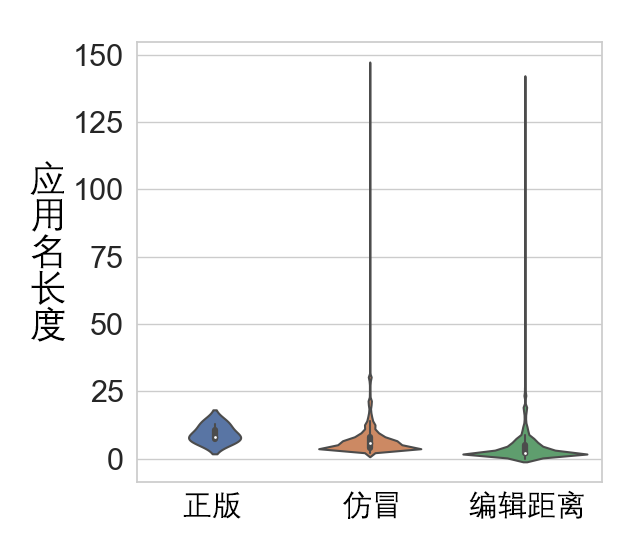
\includegraphics[width=0.333\textwidth]{./Figures/edwin-RQ1-2(a).png}}\hfill
    \subfloat[包名\label{fig:pkgname}]{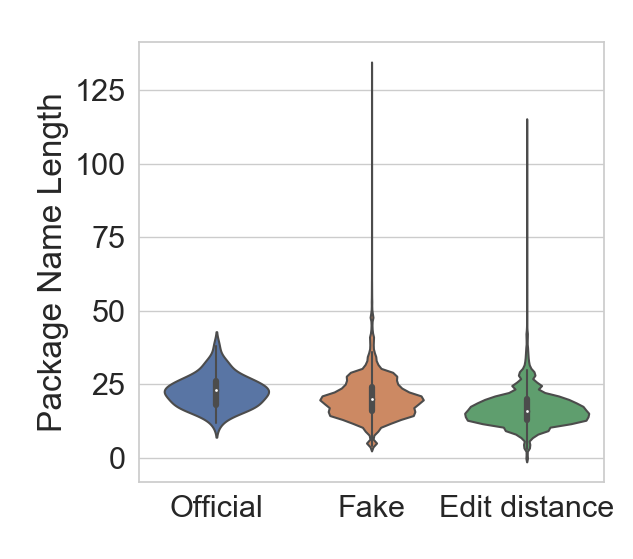
\includegraphics[width=0.333\textwidth]{./Figures/edwin-RQ1-2(b).png}}\hfill
    \subfloat[样本大小\label{fig:size}]{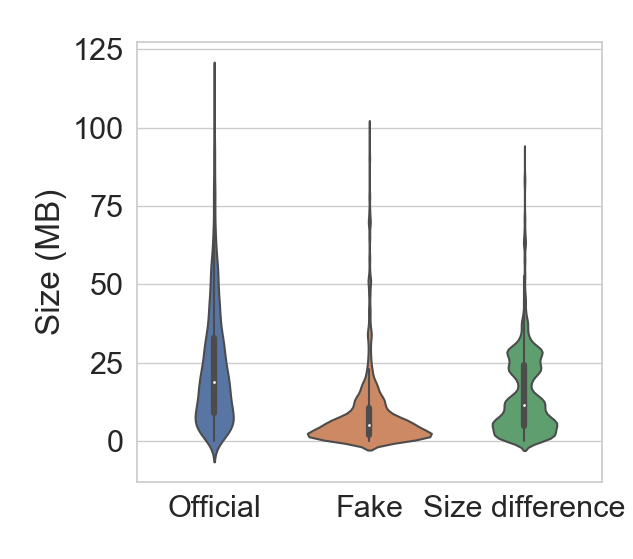
\includegraphics[width=0.333\textwidth]{./Figures/edwin-RQ1-2(c).png}}\hfill
    \caption{应用的应用名、包名与应用大小的相似性比较}
    \label{fig:Statistic_fake_and_official}
    \vspace{-5mm}
\end{figure*}

\autoref{fig:Statistic_fake_and_official}由三个小提琴图~\cite{violinplot}组成,分别表示了本文在应用名、包名和APK包大小上的统计信息。
每个``小提琴''的外部形状为数据的密度分布情况,小提琴中间的黑色粗条表示四分位数范围,粗条中小白点表示数据的中位数,黑色细条表示95\%置信空间范围。

\autoref{fig:appname}从左到右的三个图例分别展示官方样本、仿冒样本的应用名和两者间编辑距离的统计数据。
其中``正版''图例和``仿冒''图例中的中位数标志都接近数值``6'',说明官方样本和仿冒样本的应用名的平均长度十分相近。
``仿冒''图例整体分布具有集中性,较多样本分布在$y$轴数值为4到5之间,说明较多仿冒样本应用名长度落于此区间内。
``编辑距离''图例外部形状与``仿冒''图例大致类似,中位值十分低(在$y$轴上为``2''),意味着过半数仿冒应用通过从官方App的应用名中修改少于3个字符来获得其应用名。
上述结果表示大部分仿冒应用正在使用与官方App非常相似的应用名。
将三个图例与前文统计数据结合,可推断具备不同应用名的10,775个仿冒样本多数在原版应用名的基础上删减少量字符以获得新应用名。
同时,极少量仿冒应用有着异乎寻常的长名称(11个仿冒样本的应用名长度大于50个字符,最长的仿冒样本的应用名中甚至有146个字符)。
作者认为这部分异常样本可能是出于测试市场审查机制的目的被上传的。
此外,作者对部分具有长应用名的仿冒样本进行人工检查,一些长应用名拼合了多个热门App的名称(比如``潮流女装-美丽说蘑菇街淘宝天猫京东美团精选''或``老黄历万年历日历-农历天气预报知乎倒数日记账事本闹钟备忘录优步滴滴打车同花顺大智慧微博大众点评小说壁纸'')。
这可能是为了应用更容易地被用户搜索到而采取的策略。

\autoref{fig:pkgname}显示了针对包名的结果。
官方App的包名长度中位值和仿冒样本的包名长度中位值较为接近(双方的值分别为``23''和``20''),两者外形较为近似,说明原版样本与仿冒样本在包名长度上有类似分布。
然而,原版包名与仿冒样本包名之间编辑距离的中位数明显较高(在$y$轴上``16''的位置),这意味着将一个仿冒应用的包名转换为一个官方App的包名平均需要进行16次编辑。
换言之,官方App的包名和仿冒应用的包名有明显差异,仿冒应用更倾向于使用自定义且与原版应用有较大区别的包名。

\autoref{fig:size}则显示APK包大小的相关对比。
为了能更好地显示结果,部分极端样本在作图前被剔除出数据集:该部分样本为大于150MB的APK包,在所有69,614个官方App的样本中占851个(约为1\%),在52,638个仿冒样本中占447个(少于1\%),大部分来源于``游戏''类别下。
图表显示,仿冒样本大小的中位数约为5MB,约半数的正版App大小大于18MB。
``正版''图例中,应用大小样本分布相对均匀,密度曲线变化平缓,大部分样本分布于$(0, 60)$MB区间内,多数正版应用大小小于25MB,但在大于25MB的区间内仍有少量样本分布;
与之相比,``仿冒''图例的样本分布集中于3到4MB处,几乎没有样本大小大于25MB;
从该角度看,仿冒应用更有可能:

1) 由仿冒开发者自行开发,而非使用重打包技术制作。因为重打包之后的应用通常不会在大小上与原版有太大差距;

2) 是恶意应用。单独的恶意应用不需要包括较大的资源文件,只需少量具备恶意代码即可产生恶意行为;

\vspace{1mm}

简而言之,可从\autoref{fig:Statistic_fake_and_official}中获得两点总结,回答RQ1:

1) 更倾向于使用与正版App相似(甚至相同)的应用名,但包名与正版应用相差较大;

2) APK大小通常较小,很可能为仿冒应用开发者重新开发的恶意应用。
\vspace{1mm}


\begin{figure*}[t]
    \centering
    \subfloat[360应用市场\label{fig:360_detail}]{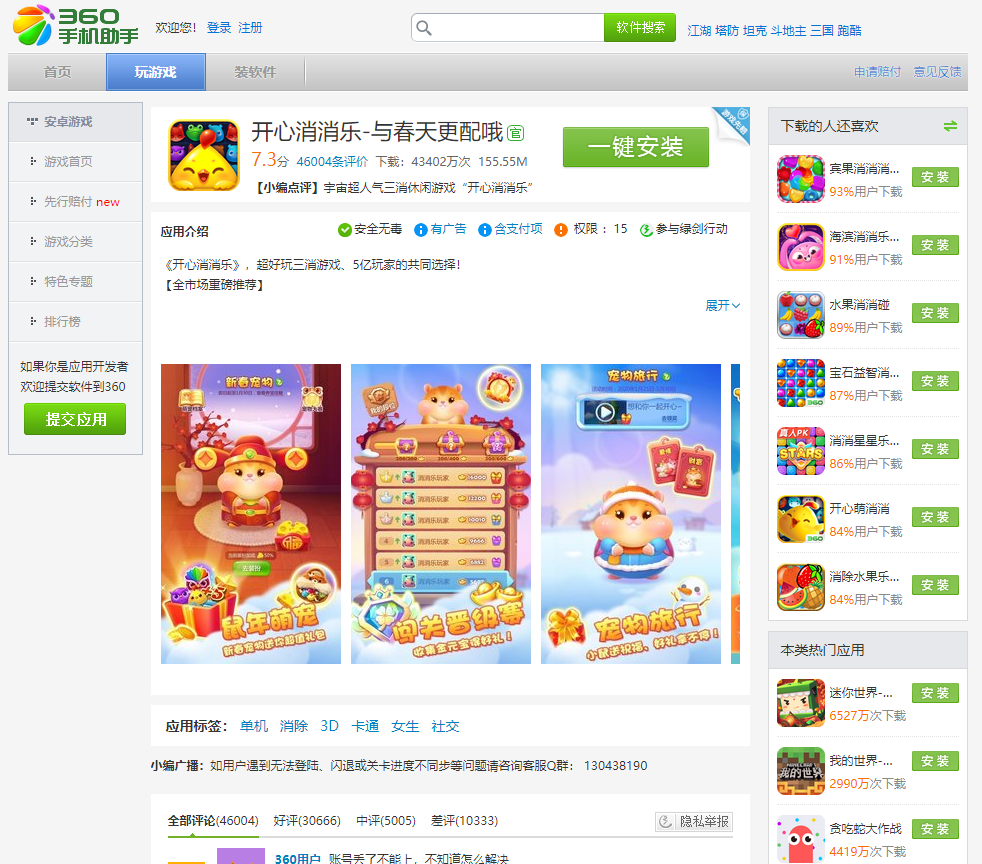
\includegraphics[width=0.49\textwidth]{./Figures/edwin-app-detail-360.png}}\hfill
    \subfloat[应用宝\label{fig:yyb_detail}]{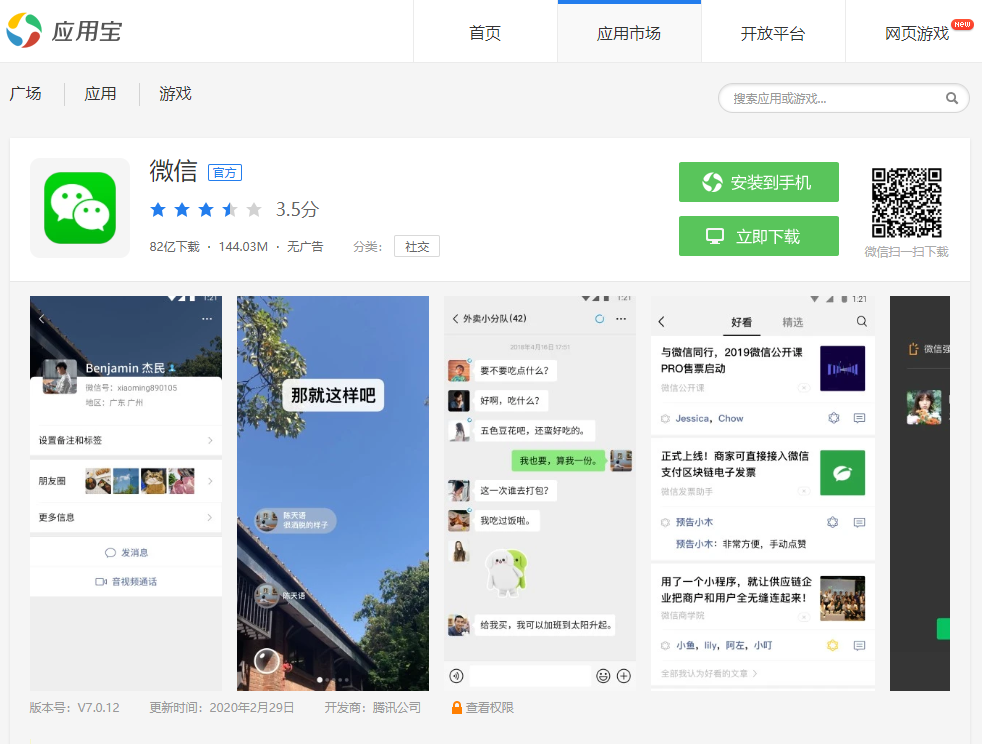
\includegraphics[width=0.49\textwidth]{./Figures/edwin-app-detail-yyb.png}}\hfill

    \subfloat[百度手机助手\label{fig:baidu_detail}]{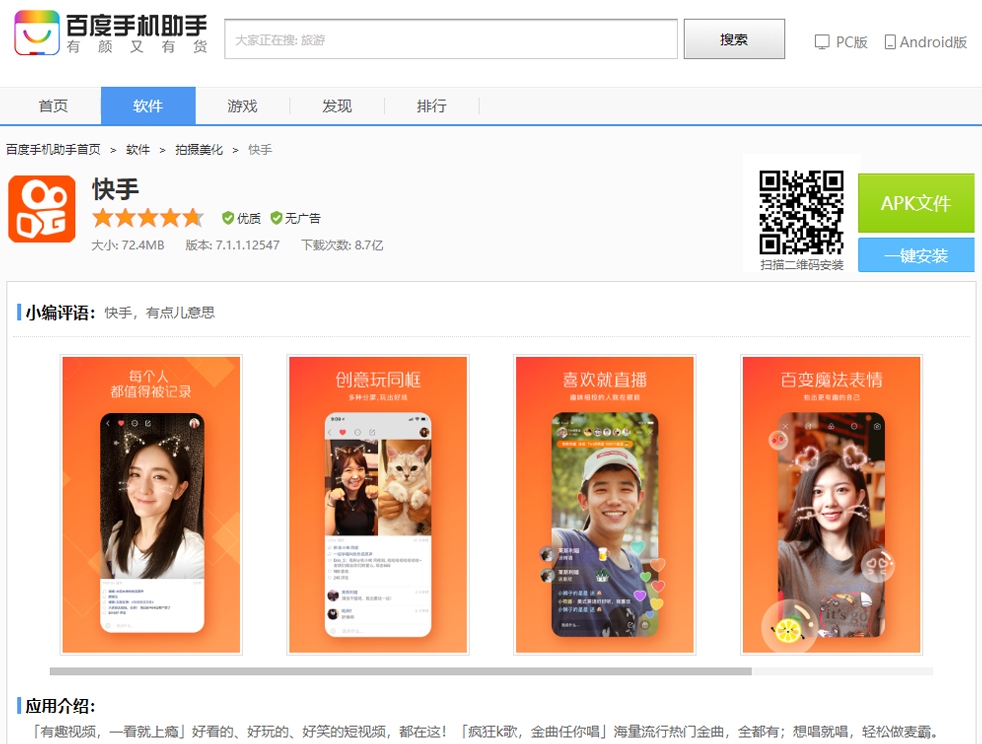
\includegraphics[width=0.49\textwidth]{./Figures/edwin-app-detail-baidu.png}}\hfill
    \subfloat[小米应用市场(部分信息被折叠)\label{fig:xiaomi_detail}]{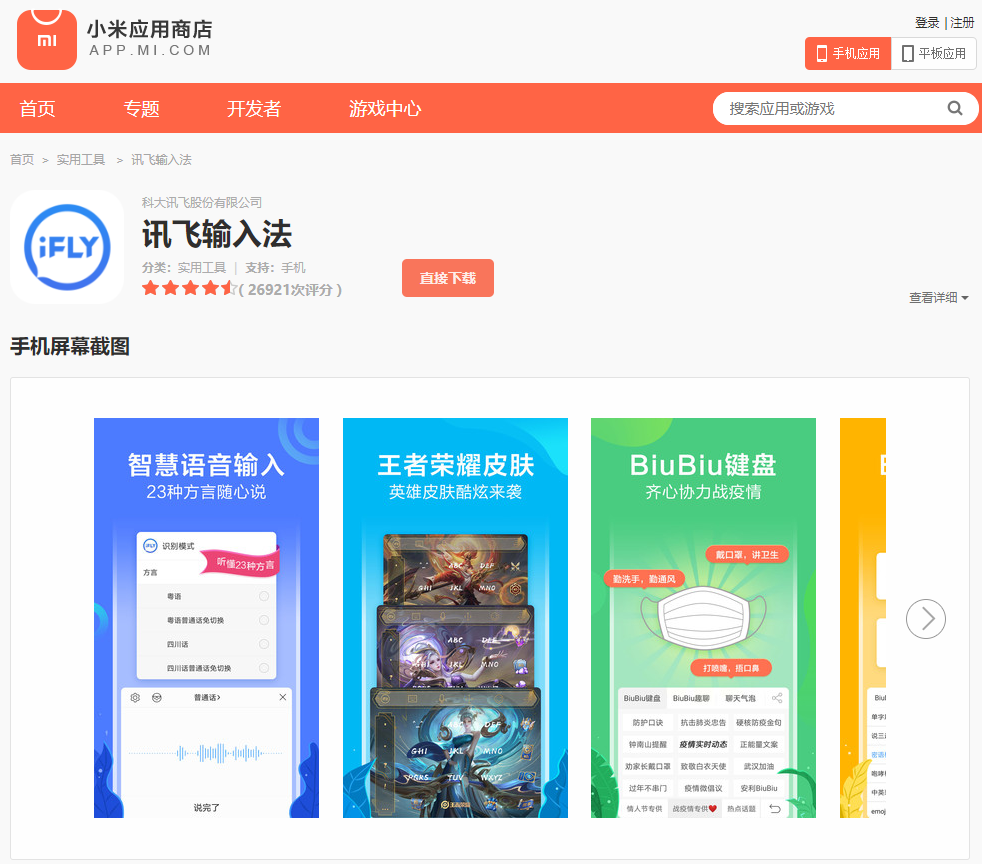
\includegraphics[width=0.49\textwidth]{./Figures/edwin-app-detail-xiaomi.png}}\hfill
    \caption{各大应用市场应用详情页}
    \label{fig:app_detail_page}
    \vspace{-5mm}
\end{figure*}

作者认为,造成上述第一点总结的原因是应用市场上提供的应用信息的不完备和用户对Android App了解的缺乏。
\autoref{fig:app_detail_page}显示了4个国内主流应用市场的详情页。
当用户浏览应用详情页时,各应用市场均显示对应应用的应用名、下载量、应用描述、其他用户对应用的评论和评分等信息。
但是,页面上较为醒目的条目是应用名、应用评分和图标信息,应用的技术参数(比如应用大小、版本号等)信息或是在不显眼处标记,或是被折叠,甚至不被展示。
在\autoref{fig:xiaomi_detail}所示的小米应用市场上,用户不能直接看到应用大小信息,需要点开折叠页才能获得相关数据。
上述四个应用市场应用详情页均不显示应用的包名信息。
由于普通用户不了解Android App中包名和应用名的区别和关联,展示相关信息对市场方引导用户下载安装应用也没有促进作用,市场对应用的技术参数展示并不重视。
因此,用户在应用市场上无法感知应用包名甚至应用大小,仿冒应用开发者无需在该两点上花费精力模仿正版应用。
相反,一方面,应用名在市场详情页上处于显眼位置,仿冒应用名称与正版越接近,越容易误导用户下载;另一方面,应用名重名不会在技术上造成阻碍。
因此,仿冒应用的应用名与正版应用十分类似,但包名、应用大小与正版应用相距较大。

\subsection{影响应用被仿冒的严重程度的因素}
\label{sec:quantitativeStudy}

\noindent{\bf RQ2:是否存在显著影响应用被仿冒的严重程度的单一因素?}

影响应用被仿冒的严重程度的因素众多,如能找到影响应用被仿冒的严重程度的主要因素,可针对性地制订策略防范仿冒应用。
根据经验,监管严格的应用市场上,仿冒应用更难通过审核;
一个应用的热度越高,越可能被仿冒应用开发者抄袭;
不同类别的应用具有不同目标人群,也可能影响仿冒应用开发者对其的态度。
因此,作者假设仿冒应用的数目与其来源市场相关,也受原版应用的热度、应用分类等因素影响。
App的更新频率也被视作影响仿冒数量的潜在因素,因为频繁更新的App或许可阻碍仿冒应用开发者对其进行仿冒。
根据上述因素,分别从应用所在市场与应用自身出发,作者将RQ2再细分为以下子问题:

{\bf RQ 2.1}:仿冒应用主要源于什么市场?仿冒率与市场规模是否有关系?

{\bf RQ 2.2}:某应用的热度/更新频率/所在类别是否影响其对应仿冒率?

\noindent{\bf RQ 2.1}:仿冒应用主要源于什么市场?仿冒率与市场规模是否有关系?

本研究中搜集的应用样本来源于多个不同的应用市场,不同市场规模不一,其审核、监管力度也并不一致。
根据各个样本的来源,有统计结果如\autoref{fig:Sample_source}。

\begin{figure*}[htbp]
    \centering
    \setlength{\belowcaptionskip}{-10pt}
    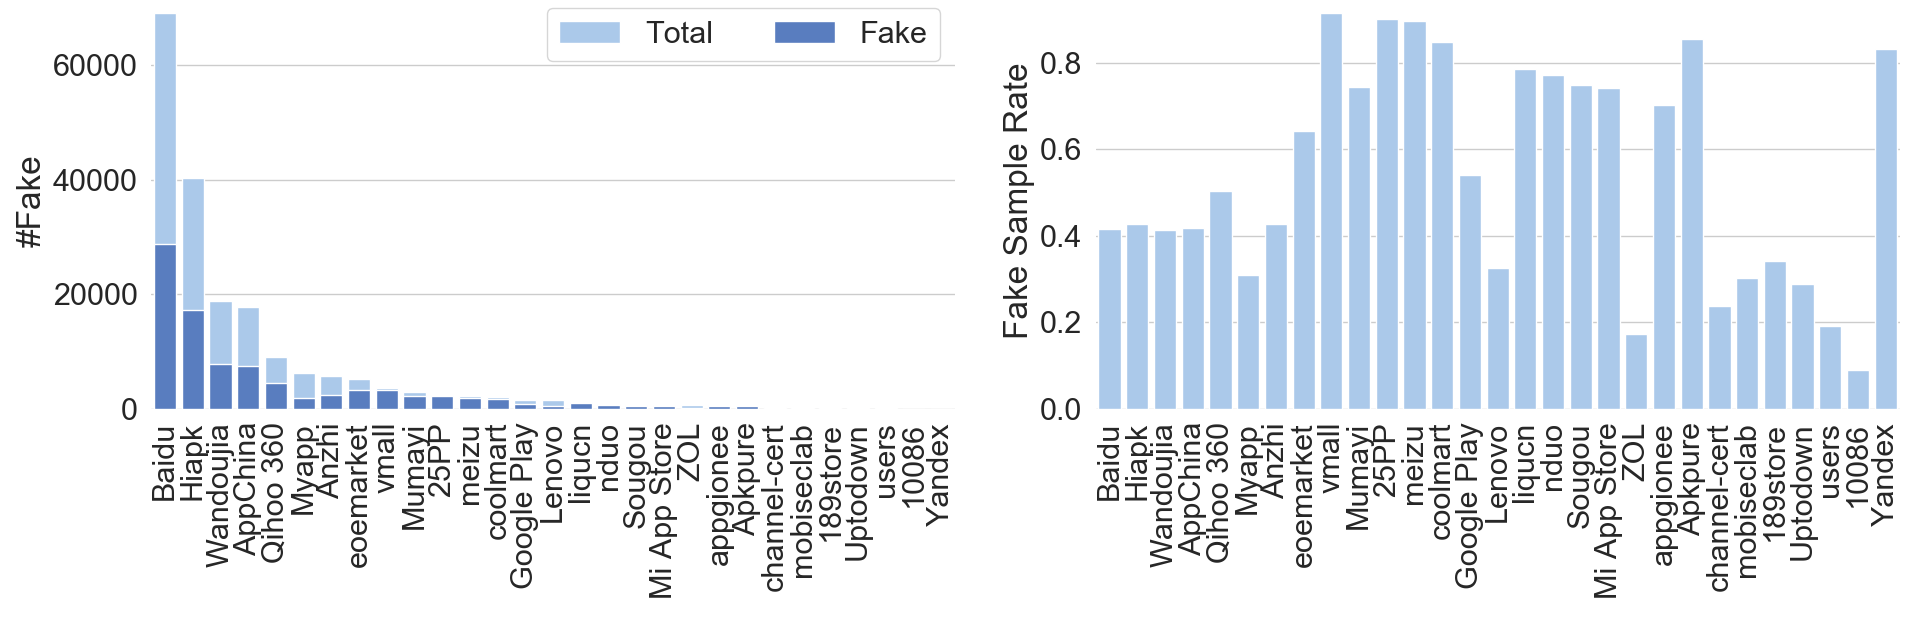
\includegraphics[width=\textwidth]{./Figures/edwin-Number_of_samples_collected_markets_3.png}
    \caption{从不同应用市场中收集到的应用数量以及各市场仿冒率}
    \label{fig:Sample_source}
\end{figure*}

左图显示,在本研究收集数据的所有29个应用来源中,从样本总数与仿冒样本数两个角度看,\texttt{百度手机助手}均提供了最多样本。
由于本研究选取的目标应用为市面上最受欢迎的应用,较有代表性,可将各渠道提供的样本量与国内市场规模相联系。
各个应用市场的仿冒率在右图呈现。


\texttt{百度手机助手}~\cite{Baiduappstore}和\texttt{安卓市场}~\cite{Hiapk}的仿冒率均约为40\%,在所有的29个渠道中处于中等水平,但由于源于该两个渠道样本基数最大,两者也提供了最多仿冒样本数。
由图中数据可得,应用市场的样本数量与仿冒率不直接相关。
然而,应用和市场的关系有可能对应用仿冒率产生影响:
本研究的50款目标应用中,有12款由腾讯公司开发,3款由360开发。
针对该15款应用进行仿冒率计算,得到各应用于规模较大的9个应用市场中仿冒率如下:

\begin{table}[htbp]
    \renewcommand{\arraystretch}{1}
    \footnotesize
    \centering
    \caption{15款应用于各大市场的仿冒率(数值单位:\%)}
    \vspace{1mm}
    \begin{tabular}{l c c c c c c c c c}
        \toprule
                                        & {\bf 百度} & {\bf 安卓市场} & {\bf 豌豆荚} & {\bf 应用汇} & {\bf 360} & {\bf 应用宝} & {\bf 安智} & {\bf 优亿} & {\bf 华为} \\
        \midrule
        QQ                              & 54.86      & 52.73          & 49.74        & 46.12        & 49.45     & 29.72        & 26.36      & 66.55      & 95.73      \\
        \rowcolor{gray!15} 微信         & 89.94      & 90.47          & 93.6         & 89.05        & 92.34     & 53.19        & 94.58      & 95.0       & 99.81      \\
        腾讯视频                        & 6.25       & 4.55           & 13.27        & 10.84        & 4.55      & 0.0          & 2.0        & 0.0        & 66.67      \\
        \rowcolor{gray!15} 腾讯手机管家 & 62.9       & 78.94          & 72.14        & 67.29        & 82.67     & 56.32        & 74.74      & 87.1       & 98.04      \\
        QQ音乐                          & 5.09       & 2.04           & 12.87        & 5.71         & 2.63      & 1.96         & 0.0        & 19.35      & 84.21      \\
        \rowcolor{gray!15} 开心消消乐   & 89.66      & 80.19          & 87.5         & 47.89        & 70.23     & 63.54        & 66.67      & 93.7       & 96.36      \\
        王者荣耀                        & 83.91      & 78.84          & 66.19        & 55.88        & 77.42     & 28.92        & 67.21      & 93.15      & 88.89      \\
        \rowcolor{gray!15} QQ邮箱       & 2.37       & 1.72           & 0.0          & 6.06         & 0.0       & 0.0          & 0.0        & 15.38      & 66.67      \\
        QQ浏览器                        & 2.18       & 2.47           & 10.78        & 1.98         & 6.52      & 0.0          & 2.7        & 15.79      & 90.0       \\
        \rowcolor{gray!15} 腾讯新闻     & 0.82       & 1.31           & 0.0          & 5.56         & 0.0       & 0.0          & 0.0        & 0.0        & 0.0        \\
        应用宝                          & 39.63      & 56.12          & 22.01        & 28.39        & 44.68     & 52.38        & 92.86      & 80.0       & 91.43      \\
        \rowcolor{gray!15} 全民K歌      & 42.86      & 43.01          & 35.78        & 55.77        & 60.38     & 23.81        & 49.06      & 35.29      & 66.67      \\
        360手机卫士                     & 65.92      & 46.2           & 79.56        & 74.78        & 67.27     & 91.46        & 82.05      & 83.08      & 96.1       \\
        \rowcolor{gray!15} 360清理大师  & 4.26       & 6.67           & 0.0          & 13.04        & 0.0       & 0.0          & 0.0        & 9.09       & 0.0        \\
        360手机助手                     & 33.89      & 68.0           & 17.89        & 45.21        & 19.48     & 30.0         & 37.5       & 15.79      & 87.5       \\
        \bottomrule
    \end{tabular}
    \label{table:firm_apps}
\end{table}

腾讯系的12款应用分别为QQ,微信,腾讯视频,腾讯手机管家,QQ音乐,开心消消乐,王者荣耀,QQ邮箱,QQ浏览器,腾讯新闻,应用宝和全民K歌;
360系的3款应用为360手机卫士,360清理大师和360手机助手。
应用宝为腾讯旗下应用市场,~\autoref{table:firm_apps}中结果表明,应用宝中腾讯系应用仿冒率明显比其他市场低;
同样地,360系应用在360市场中的仿冒率也比其他市场中明显降低。
作者猜测,应用宝对12款腾讯系应用相关的应用有较为严格的审核流程,有效遏制了该市场中与上述12款腾讯系应用相关的仿冒应用。
同理,360系应用在360市场中仿冒率较低。

结果表明,应用市场的规模与仿冒率无明显关联,但应用本身与市场的关系对仿冒率有影响。

\noindent{\bf RQ 2.2}:某应用的热度/更新频率/所在类别是否影响其对应仿冒率?

通常,某款App越受欢迎,其对应的仿冒应用越有可能被用户误下载,令仿冒应用开发者获取利润,吸引更多仿冒应用开发者对其仿冒;
应用更新可被分为功能性更新与安全性更新两类,频繁更新的应用功能迭代速度快,复杂度高,也可能有更好的安全性,使仿冒开发者难以复刻;
不同类别的应用具有不同目标人群与功能,也可能影响对应的应用被仿冒的严重程度。
针对上述前两个因素,本节使用皮尔逊积矩相关系数衡量仿冒率与因素对应维度指标的关联性;由于类别无法用连续变量表示,相关系数不适用于该因素,本研究将以图表形式表示两者之间的关联程度。

热度数据源于易观千帆平台;
应用更新频率取自某应用最早版本与最新版之间的平均更新时长,即两者发行时间差值与中间版本数的商;
根据应用功能划分,本研究的50款目标应用被分为11个类别,分别为应用市场,摄影录像,游戏,资讯,生活,音乐,移动购物,商务办公,社交网络,系统工具,视频。

\begin{ThreePartTable}
    \centering
    \renewcommand{\arraystretch}{1.05}
    \footnotesize
    \setlength{\belowcaptionskip}{-5pt}
    \vspace{1mm}
    \begin{longtable}{l l c c c c c c}
        \caption{目标应用与其相关统计}\label{table:data-statistics}                                                                                                                                      \\
        \toprule
        {\bf 应用名}                    & {\bf 类别} & \begin{tabular}[c]{@{}c@{}}{\bf 月度热} \\ {\bf 度指数} \end{tabular} & \begin{tabular}[c]{@{}c@{}}{\bf 更新频率} \\ {\bf (天/版本)} \end{tabular} & {\bf 样本总数} & \begin{tabular}[c]{@{}c@{}}{\bf 仿冒} \\ {\bf 样本数} \end{tabular} & {\bf 仿冒率} & \begin{tabular}[c]{@{}c@{}}{\bf 平均仿冒} \\ {\bf 延迟(天)} \end{tabular} \\
        \midrule
        微信                            & 社交网络   & 91.2K                      & 6.4                        & 9248           & 6447                       & 69.7\%       & 12.1                       \\
        \rowcolor{gray!15} QQ           & 社交网络   & 54.6K                      & 10.7                       & 11167          & 3780                       & 33.8\%       & 9.2                        \\
        爱奇艺                          & 视频       & 53.5K                      & 6.4                        & 7586           & 3481                       & 45.9\%       & 9.3                        \\
        \rowcolor{gray!15} 支付宝       & 生活       & 48.1K                      & 10.2                       & 983            & 231                        & 23.5\%       & 10.1                       \\
        淘宝                            & 移动购物   & 47.5K                      & 7.0                        & 6003           & 3010                       & 50.1\%       & 8.1                        \\
        \rowcolor{gray!15} 腾讯视频     & 视频       & 47.3K                      & 6.3                        & 1429           & 68                         & 4.8\%        & 10.7                       \\
        优酷                            & 视频       & 40.9K                      & 7.3                        & 2058           & 262                        & 12.7\%       & 6.7                        \\
        新浪微博                        & 社交网络   & 39.2K                      & 5.3                        & 5947           & 2715                       & 45.7\%       & 5.7                        \\
        \rowcolor{gray!15} WiFi万能钥匙 & 系统工具   & 36.4K                      & 3.1                        & 4808           & 2999                       & 62.4\%       & 3.0                        \\
        搜狗输入法                      & 系统工具   & 33.3K                      & 11.0                       & 898            & 40                         & 4.5\%        & 21.8                       \\
        \rowcolor{gray!15} 百度         & 资讯       & 32.4K                      & 11.1                       & 15651          & 3514                       & 22.5\%       & 12.8                       \\
        腾讯新闻                        & 资讯       & 28.7K                      & 8.5                        & 1051           & 11                         & 1.0\%        & 8.9                        \\
        \rowcolor{gray!15} QQ浏览器     & 资讯       & 27.8K                      & 5.6                        & 1369           & 43                         & 3.1\%        & 11.6                       \\
        今日头条                        & 资讯       & 27.4K                      & 4.4                        & 3538           & 179                        & 5.1\%        & 5.6                        \\
        \rowcolor{gray!15} 应用宝       & 应用市场   & 27K                        & 11.4                       & 2419           & 266                        & 11.0\%       & 11.6                       \\
        快手                            & 视频       & 24.4K                      & 3.2                        & 8273           & 4270                       & 51.6\%       & 3.5                        \\
        \rowcolor{gray!15} 腾讯手机管家 & 系统工具   & 24.2K                      & 8.7                        & 2463           & 1340                       & 54.4\%       & 8.7                        \\
        高德地图                        & 生活       & 24K                        & 6.5                        & 1225           & 51                         & 4.2\%        & 13.1                       \\
        \rowcolor{gray!15} 酷狗音乐     & 音乐       & 23K                        & 8.6                        & 1313           & 122                        & 9.3\%        & 12.2                       \\
        QQ音乐                          & 音乐       & 21.7K                      & 9.4                        & 1132           & 65                         & 5.7\%        & 14.6                       \\
        \rowcolor{gray!15} 百度地图     & 生活       & 21.3K                      & 8.8                        & 2609           & 1438                       & 55.1\%       & 15.3                       \\
        抖音                            & 视频       & 19.4K                      & 11.1                       & 317            & 12                         & 3.8\%        & 8.3                        \\
        \rowcolor{gray!15} 京东         & 移动购物   & 18.5K                      & 10.9                       & 5000           & 2377                       & 47.5\%       & 12.3                       \\
        UC浏览器                        & 资讯       & 16.7K                      & 7.4                        & 4232           & 1624                       & 38.4\%       & 7.0                        \\
        \rowcolor{gray!15} 360手机卫士  & 系统工具   & 15.4K                      & 12.4                       & 3670           & 1423                       & 38.8\%       & 19.1                       \\
        全民K歌                         & 音乐       & 14.7K                      & 21.1                       & 618            & 215                        & 34.8\%       & 17.3                       \\
        \rowcolor{gray!15} 美团         & 生活       & 13K                        & 8.0                        & 4752           & 1415                       & 29.8\%       & 6.9                        \\
        拼多多                          & 移动购物   & 12.9K                      & 6.6                        & 2327           & 551                        & 23.7\%       & 7.8                        \\
        \rowcolor{gray!15} 王者荣耀     & 游戏       & 12.5K                      & 15.5                       & 2350           & 1319                       & 56.1\%       & 12.3                       \\
        美图秀秀                        & 摄影录像   & 12.4K                      & 5.4                        & 1705           & 784                        & 46.0\%       & 5.8                        \\
        \rowcolor{gray!15} 火山小视频   & 视频       & 12.2K                      & 11.9                       & 410            & 16                         & 3.9\%        & 9.6                        \\
        墨迹天气                        & 生活       & 12K                        & 4.2                        & 10081          & 7093                       & 70.4\%       & 4.7                        \\
        \rowcolor{gray!15} 滴滴出行     & 生活       & 11.8K                      & 8.6                        & 943            & 117                        & 12.4\%       & 7.0                        \\
        华为应用市场                    & 应用市场   & 11.8K                      & N/A                        & 0              & 0                          & 0.0\%        & N/A                        \\
        \rowcolor{gray!15} 开心消消乐   & 游戏       & 11.2K                      & 19.7                       & 2406           & 1738                       & 72.2\%       & 20.6                       \\
        酷我音乐盒                      & 音乐       & 11K                        & 2.9                        & 3778           & 69                         & 1.8\%        & 4.2                        \\
        \rowcolor{gray!15} 西瓜视频     & 视频       & 11K                        & 11.5                       & 866            & 100                        & 11.5\%       & 8.8                        \\
        OPPO应用商店                    & 应用市场   & 10.8K                      & N/A                        & 0              & 0                          & 0.0\%        & N/A                        \\
        \rowcolor{gray!15} 猎豹清理大师 & 系统工具   & 9.9K                       & 10.3                       & 1803           & 388                        & 21.5\%       & 13.5                       \\
        360清理大师                     & 系统工具   & 9.6K                       & 17.3                       & 327            & 8                          & 2.4\%        & 8.5                        \\
        \rowcolor{gray!15} 360手机助手  & 应用市场   & 9.2K                       & 7.6                        & 1616           & 137                        & 8.5\%        & 8.4                        \\
        WiFi管家                        & 系统工具   & 8.8K                       & 19.5                       & 1636           & 658                        & 40.2\%       & 15.7                       \\
        \rowcolor{gray!15} 讯飞输入法   & 系统工具   & 8.6K                       & 6.0                        & 1451           & 8                          & 0.6\%        & 10.1                       \\
        百度手机助手                    & 应用市场   & 8.2K                       & 11.4                       & 3849           & 437                        & 11.4\%       & 14.5                       \\
        \rowcolor{gray!15} 小米应用市场 & 应用市场   & 7.8K                       & N/A                        & 0              & 0                          & 0.0\%        & N/A                        \\
        WPS Office                      & 商务办公   & 7.4K                       & 6.0                        & 1152           & 69                         & 6.0\%        & 7.8                        \\
        \rowcolor{gray!15} 美颜相机     & 摄影录像   & 7.1K                       & 5.3                        & 1600           & 691                        & 43.2\%       & 6.3                        \\
        网易云音乐                      & 音乐       & 7K                         & 10.5                       & 616            & 6                          & 1.0\%        & 12.2                       \\
        \rowcolor{gray!15} 网易新闻     & 资讯       & 6.7K                       & 7.0                        & 1441           & 93                         & 6.5\%        & 5.0                        \\
        QQ邮箱                          & 商务办公   & 6.6K                       & 16.4                       & 520            & 11                         & 2.1\%        & 10.4                       \\
        \bottomrule
    \end{longtable}
    \vspace{-4mm}
\end{ThreePartTable}

\begin{figure*}[htbp]
    \centering
    \setlength{\belowcaptionskip}{-10pt}
    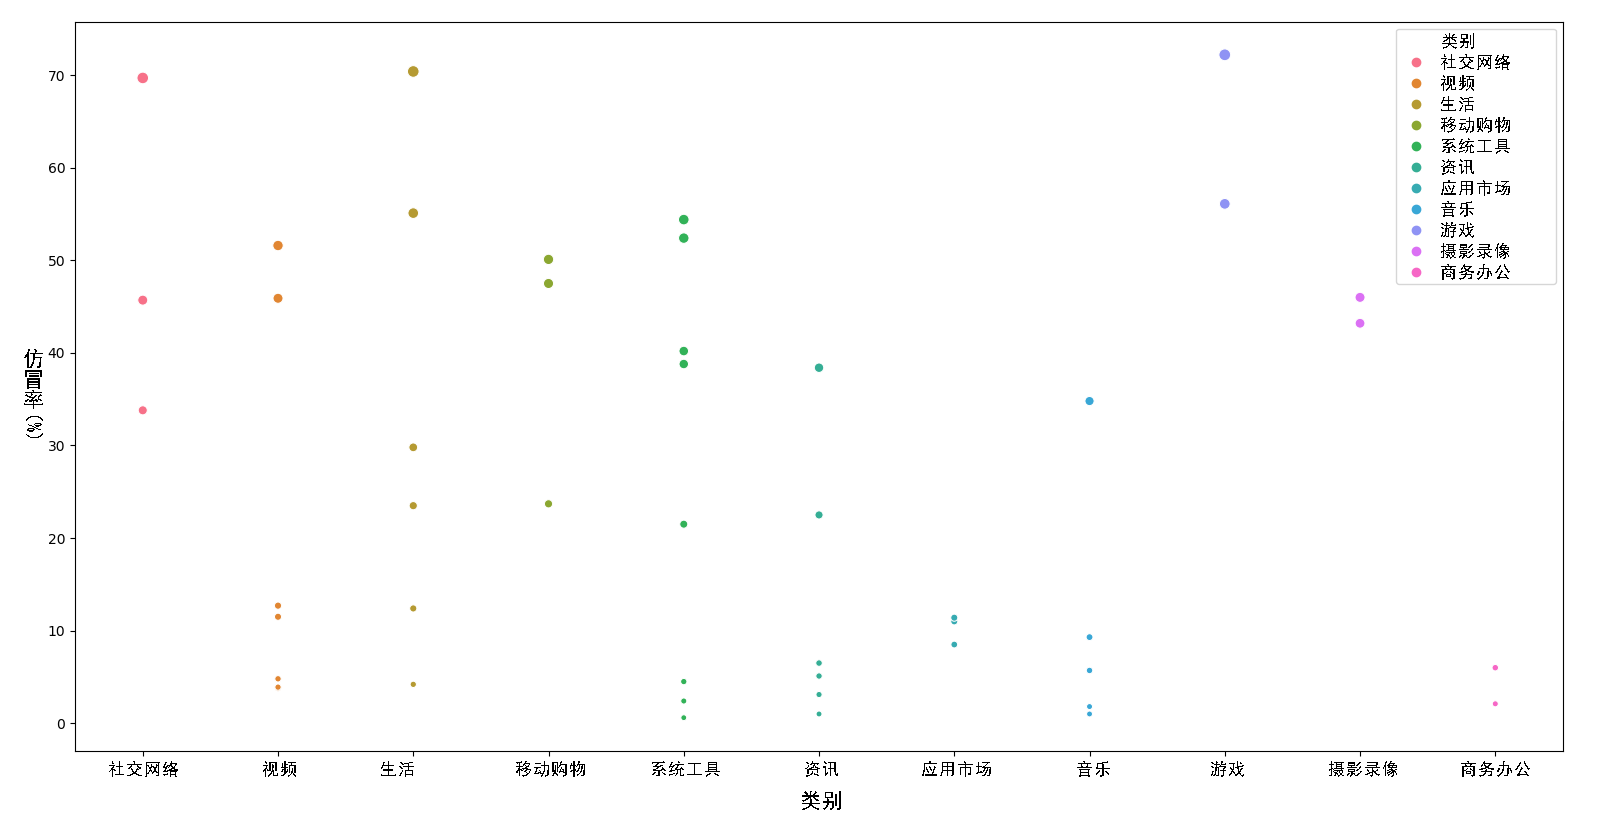
\includegraphics[width=\textwidth]{./Figures/edwin-category-fake-rate.png}
    \caption{目标应用类别-仿冒率对应图}
    \label{fig:category_fake_rate}
\end{figure*}

\autoref{table:data-statistics}按每款App的热度排序,展示了每款目标应用的类别、仿冒率、更新频率、关联样本总数等数据。
将数据代入\autoref{equ:PPMCC}可分别获得应用热度、更新频率与仿冒率之间的关联程度。
~\autoref{fig:category_fake_rate}显示每款目标应用所在类别及其仿冒率的对应关系,如$x$轴社交网络上对应的三个粉色圆点为三个社交网络类别下目标应用的仿冒率。

结果表示,仿冒率与应用热度之间的相关系数为0.246,处于较弱水平;
更新频率和仿冒率之间相关系数为0.084,两者之间几乎没有关联;
~\autoref{fig:category_fake_rate}中,除应用市场、商务办公、摄影录像、游戏四类仿冒率相对集中外,其他各类别对应应用的仿冒率较为分散。

综上,应用热度、更新频率与应用类别都不是影响应用是否会被仿冒的决定性因素,由上述结果可得:
1)应用被仿冒的的严重程度并非由单一因素决定,未来的分析应尝试从多角度同时入手分析;
2)应用更新频率与被仿冒的严重程度几乎不相关,进一步巩固了上一节的结论,即数据集中的大部分仿冒样本都不是重打包应用,而是仿冒应用开发者自行开发的。
无论官方版本受到的保护程度如何,仿冒应用开发者都可以制作对应的仿冒应用;
3)某些应用类别下的应用仿冒率相对集中,表示该类应用的确更受(或更不受)仿冒应用开发者喜爱,后续探索可从应用市场、商务办公、摄影录像、游戏四类类别入手。


\subsection{仿冒应用功能与行为}

\noindent{\bf RQ3:仿冒应用作者制作出了怎样的仿冒应用?是否依然能提供原版应用的功能?}


出于性能考虑,本研究并未对每个仿冒APK包进行详尽的拆包解析,为了解仿冒应用在功能、行为上与原版应用的差异,本研究采用案例分析的实证研究方法进行研究。
\autoref{table:data-statistics}数据显示,\texttt{游戏}类应用(\texttt{王者荣耀}和\texttt{开心消消乐})吸引了大批的仿冒应用样本。
本研究随机从这两款游戏应用的仿冒样本中各选择了7个仿冒样本与1个正版样本,将样本安装至实验设备上运行。

测试使用的设备为高配版小米5手机,搭载的CPU为最高主频2.15GHz的骁龙820处理器,3GB内存,64GB机身存储,安装的Android系统版本为Android 6.0(Android Marshmallow,API 23)。
\autoref{fig:screenshot_all}展示了这些样本在真实的Android设备上安装之后的实际外观。
官方渠道下载的正版App在图片中由绿色边框标记出。
可见仿冒应用的应用名与原版应用名十分相似,符合前文发现;仿冒应用的图标设计也与原版雷同。
本研究在测试设备上实际运行了上述安装的14个仿冒样本,将仿冒应用的界面、行为与原版应用对比,同时将样本上传至\textsc{Virustotal}~\cite{virustotal}进行恶意行为扫描。

\begin{figure}[htbp]
    \centering
    \subfloat[两种游戏App与其仿冒\label{fig:screenshot_all}]{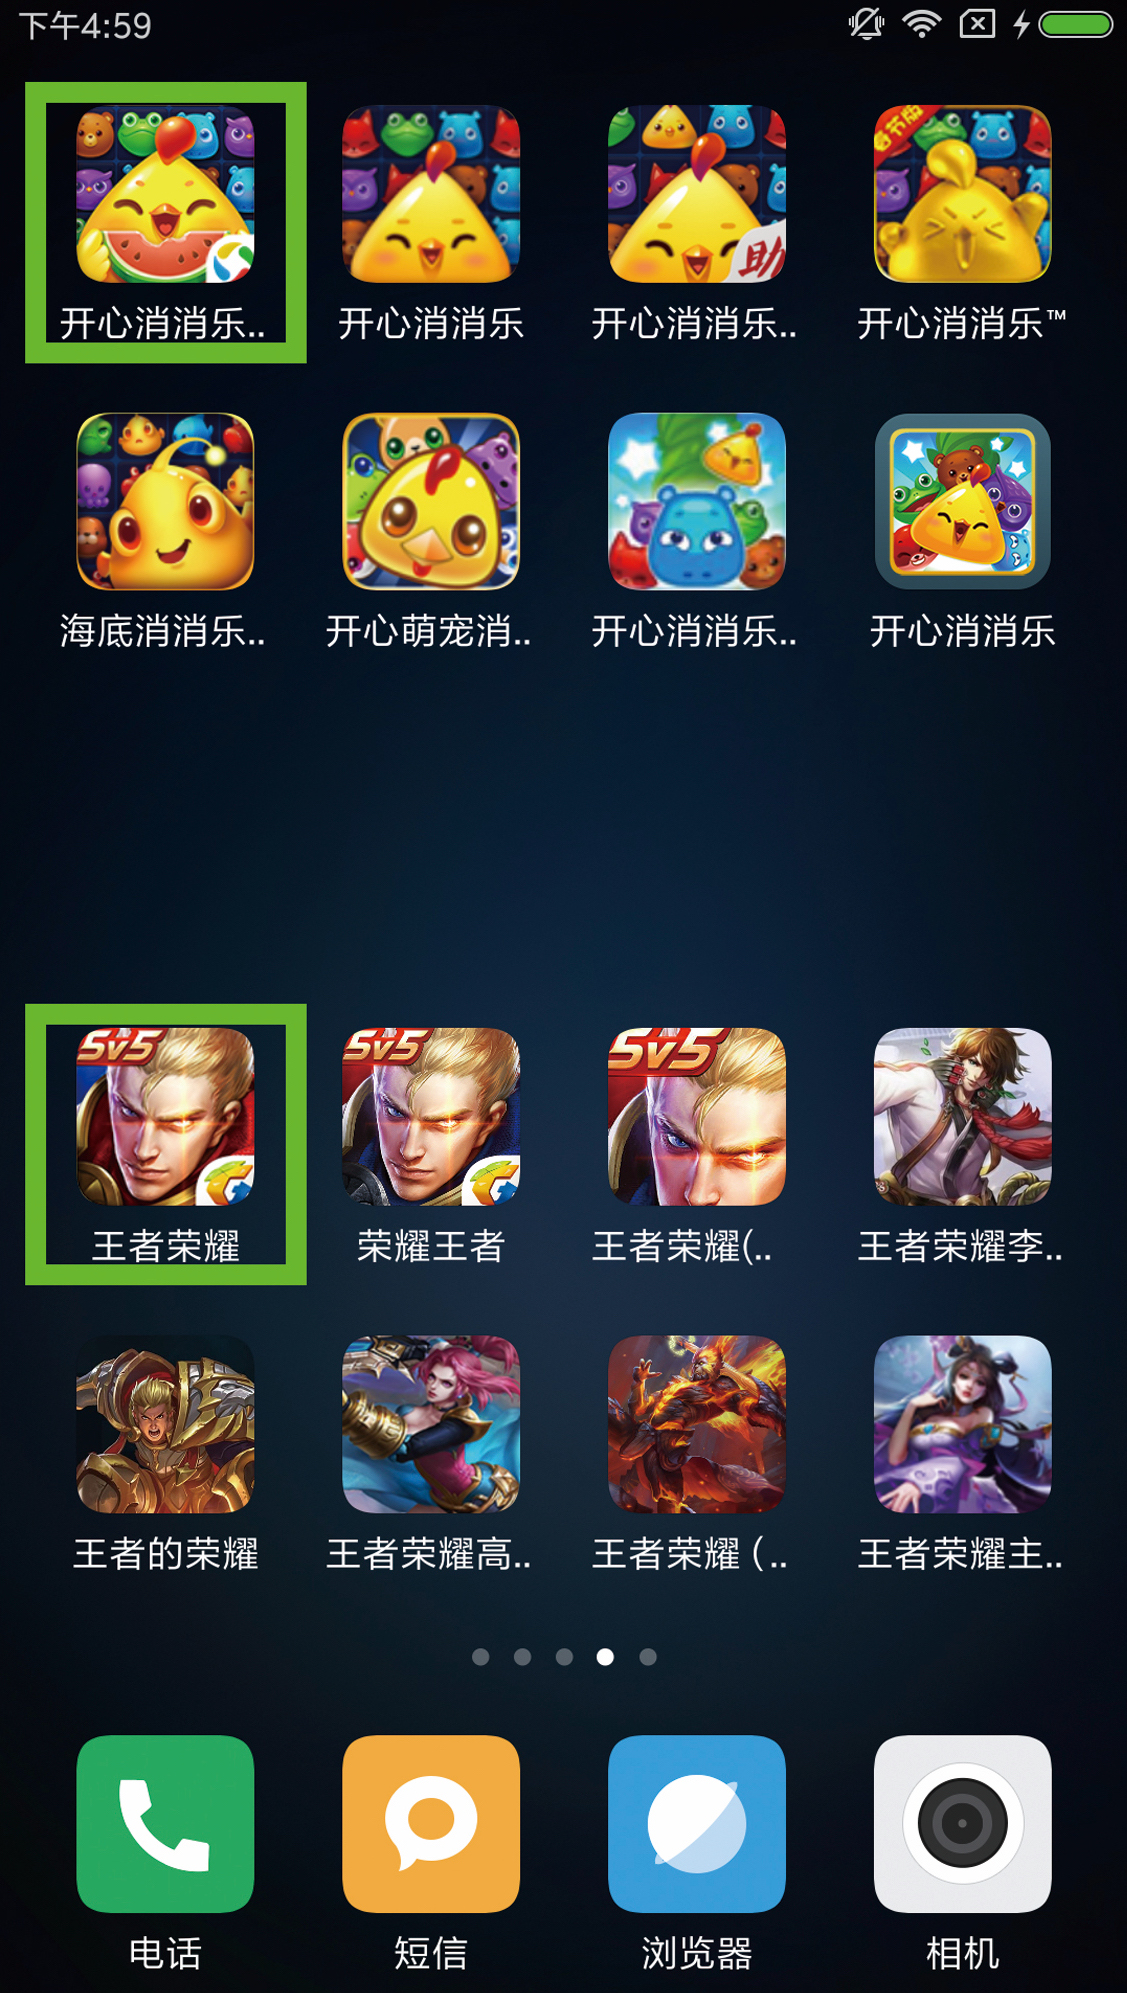
\includegraphics[width=0.3\textwidth]{./Figures/edwin-screenshot1.jpg}}\hfill
    \subfloat[正版\textit{\small 开心消消乐}\label{fig:screenshot_official}]{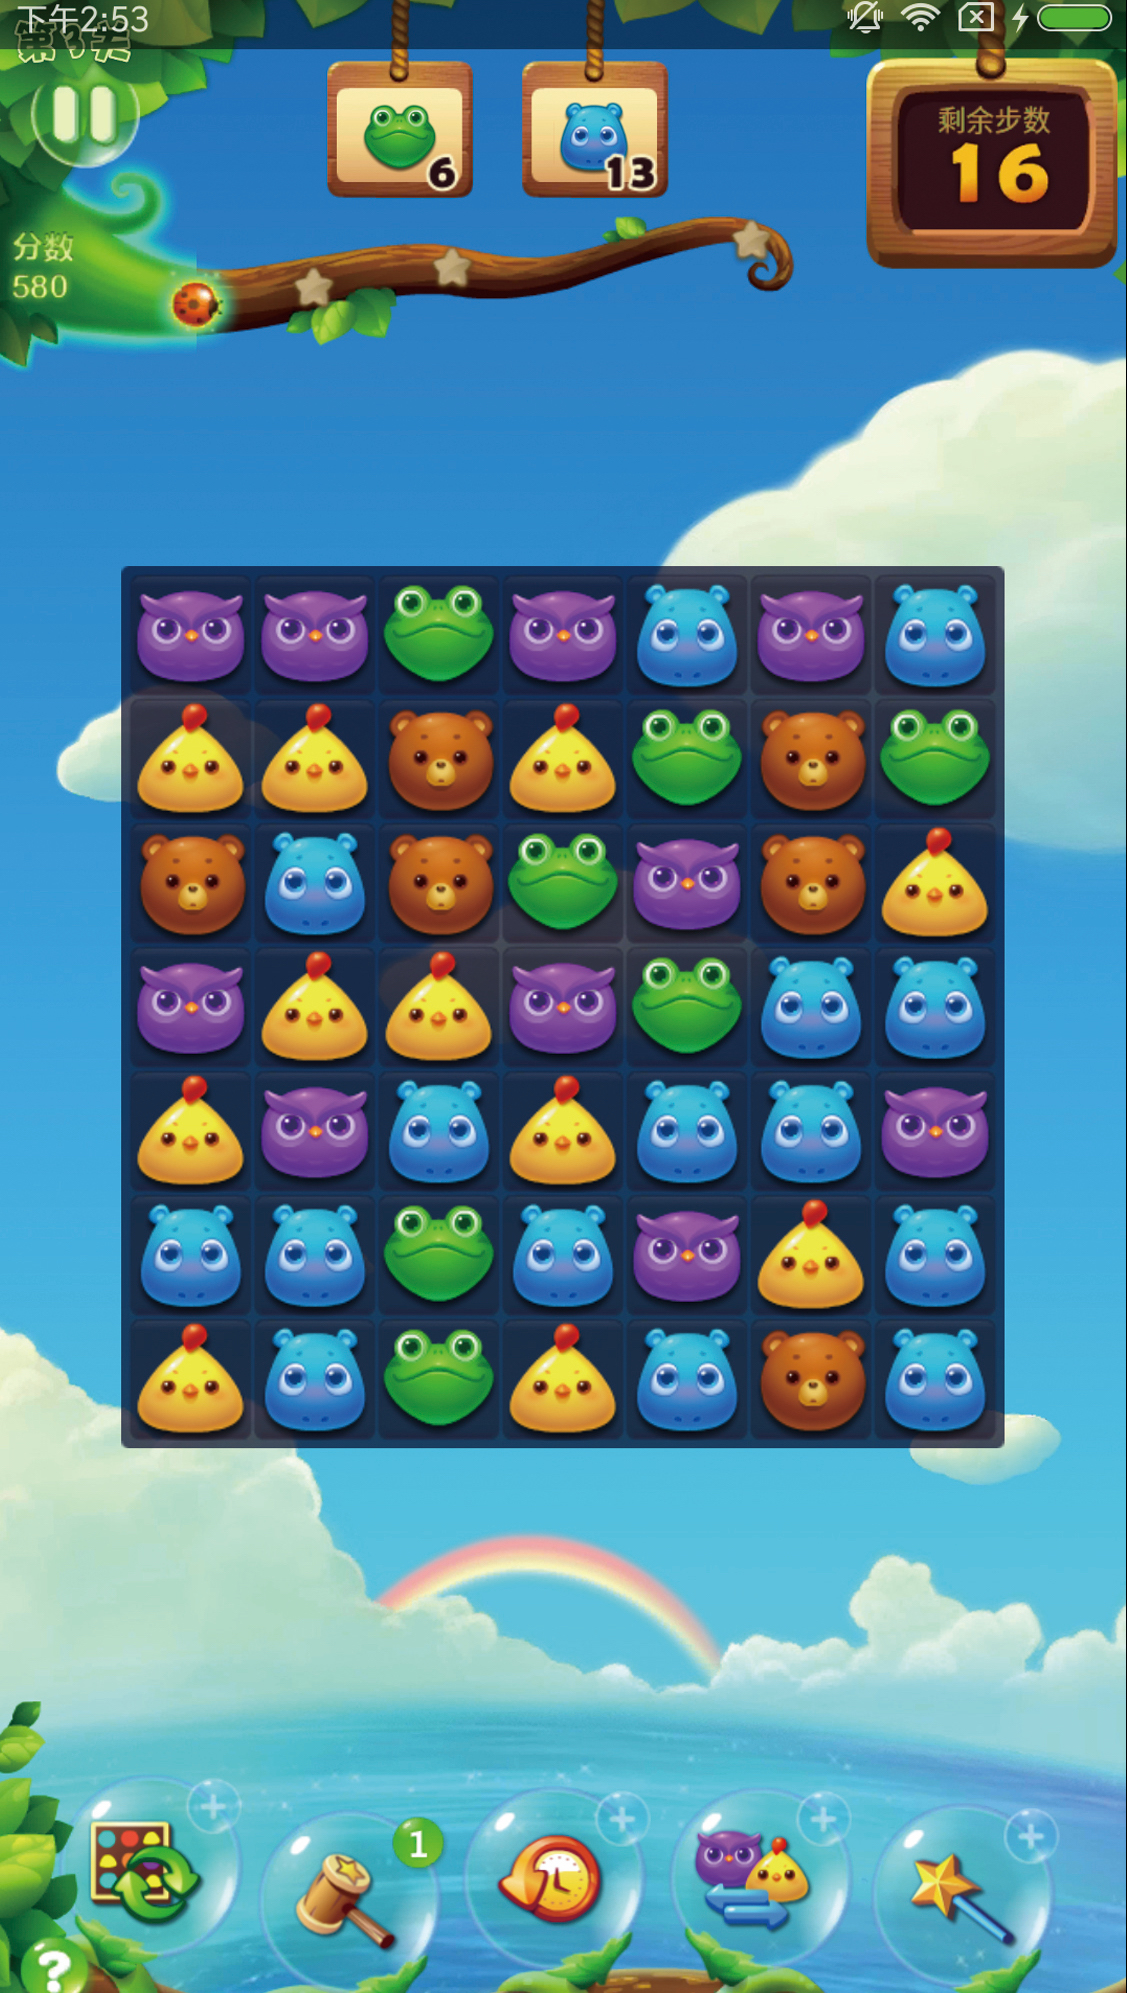
\includegraphics[width=0.3\textwidth]{./Figures/edwin-screenshot2.jpg}}\hfill
    \subfloat[仿冒版\textit{\small 开心消消乐}\label{fig:screenshot_fake}]{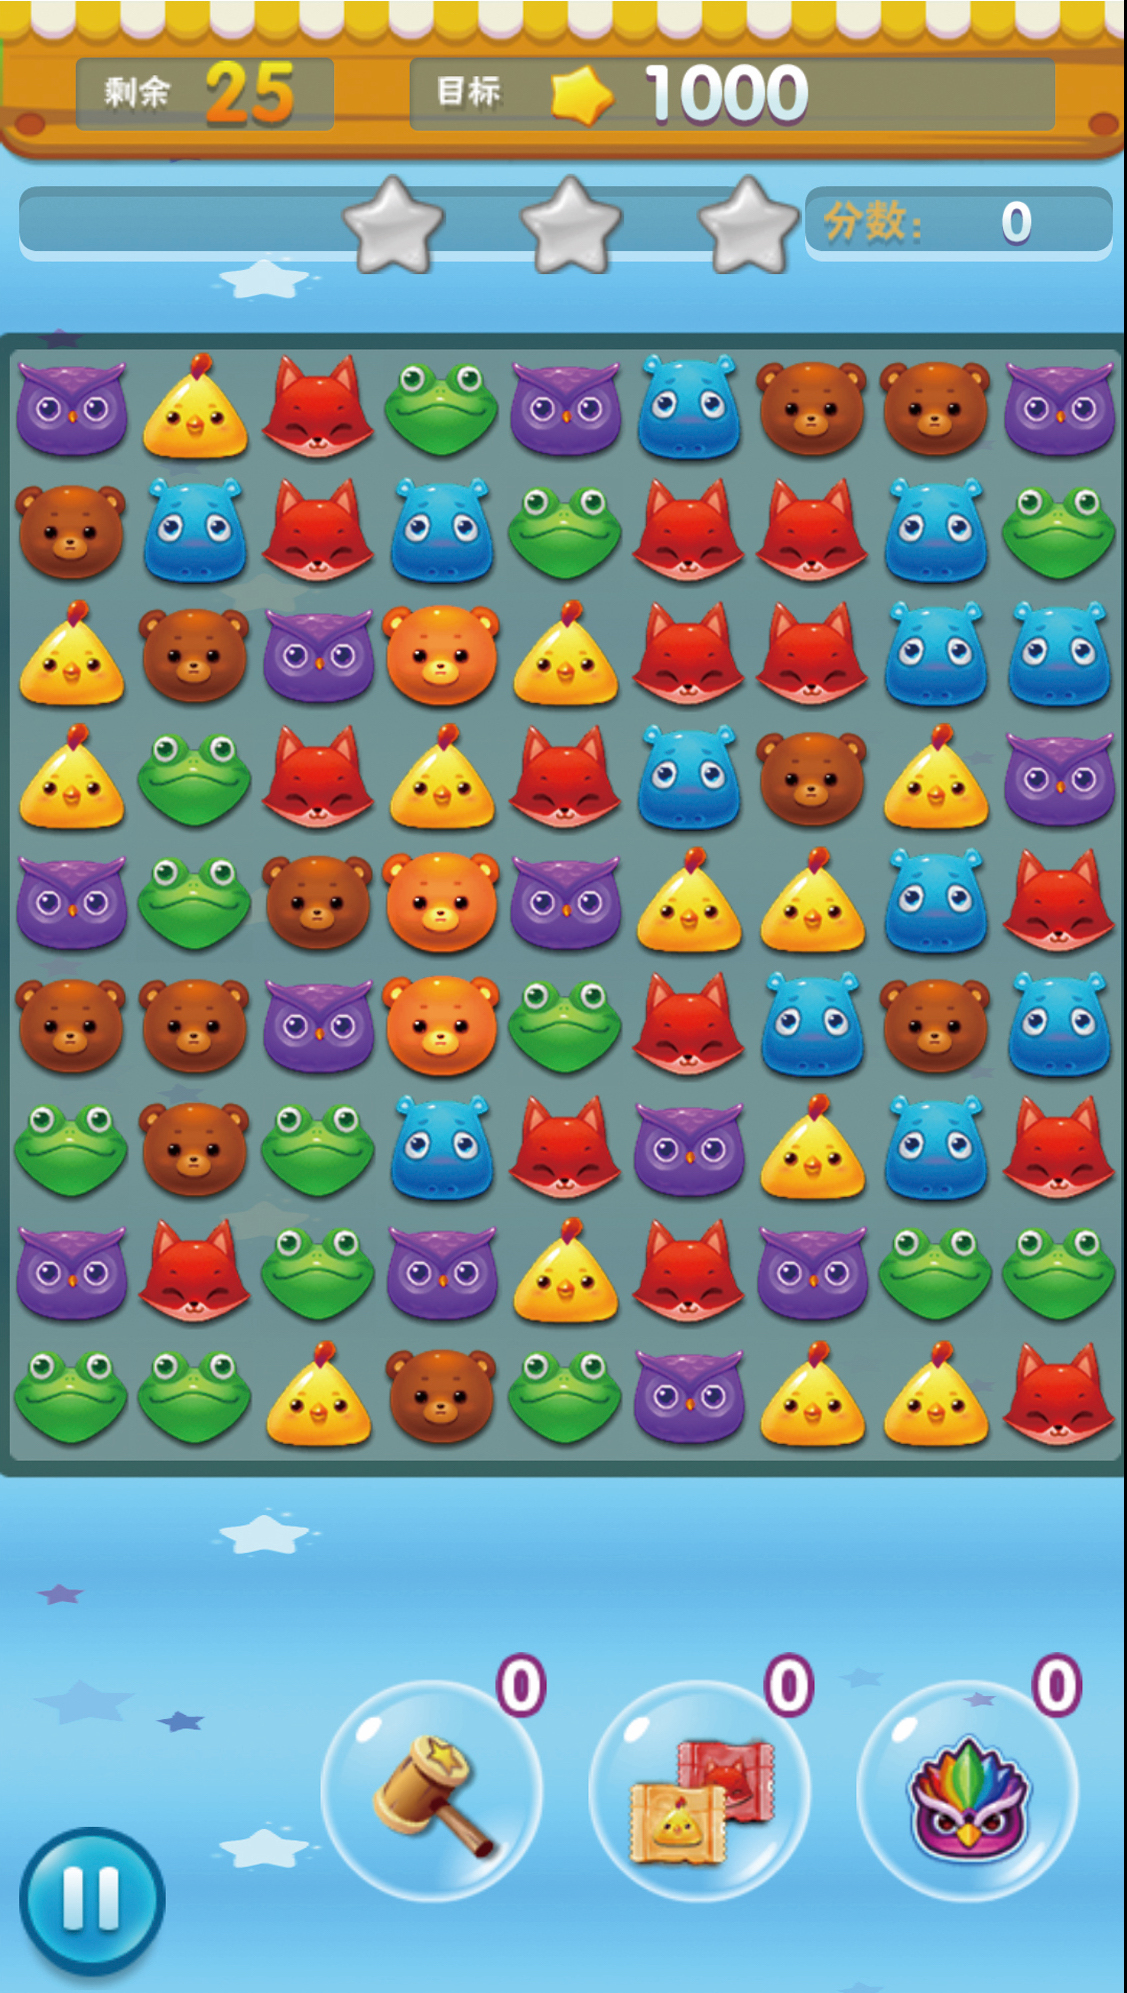
\includegraphics[width=0.3\textwidth]{./Figures/edwin-screenshot3.jpg}}\hfill
    \caption{游戏类App及其仿冒样本}
\end{figure}

\autoref{fig:screenshot_official}和\autoref{fig:screenshot_fake}分别是在测试设备上运行官方版本的\texttt{开心消消乐}和其中一个仿冒版的\texttt{开心消消乐}时的系统截屏。
从UI布局上看,两款应用的外观十分相像。
同时,仿冒版的确实现了完整的游戏功能,与正版的玩法、实际操作逻辑一模一样,有较强迷惑性。
应用开发者未必可判别两个应用的真伪,应用市场的普通用户更难以区分两者。

7款\texttt{开心消消乐}的仿冒样本中,4款与官方样本十分相似(其中之一可能是经过重打包技术处理的应用),2款声称自己是``系统攻略'',1款在运行时闪退,无法在测试设备上实际运行。
在4款仿冒游戏中,3款都在游戏中不时自动弹出游戏内购窗口,要求玩家购买道具,十分可能导致玩家不想要的花费。
所有7个仿冒样本都在\textsc{Virustotal}中被报告为恶意应用。

另一方面,\texttt{王者荣耀}的仿冒样本功能截然不同。
7款仿冒样本中,3款是壁纸浏览器,内含游戏人物插画,可在应用内将插画设置为系统壁纸;
余下4款是简单的拼图游戏,同样包含游戏人物的插画,应用内容为把被打乱的插画拼图恢复原状。
\textsc{Virustotal}显示,7款仿冒样本中,有6款是恶意软件,涵盖了木马病毒、广告软件等类型,而余下的一款则被报告为PUP(Potentially Unwanted Program,潜在有害程序)。
PUP通常在用户不知情或者不愿意的情况下,通过静默安装或者捆绑安装的形式被安装在系统中。
该类软件不一定包含恶意代码,但动机存疑。

造成该现象的原因为模仿正版应用功能难易程度不一。
从技术角度看,\texttt{王者荣耀}的设计、实现难度均比单机益智类游戏如\texttt{开心消消乐}高许多。
多人在线竞技游戏物理引擎之外,还要实现聊天系统、在线匹配、负载均衡等业务模块;
相比之下,益智类游戏的核心逻辑较为简单,无需设计多个复杂模块。

因此,即使不考虑维护问题,开发复杂游戏的成本对仿冒应用开发者而言也明显过高。
但由于\texttt{王者荣耀}的高热度可能带来巨大收益,仿冒应用开发者会为了蹭上热度而开发外观相似、内容完全不符的仿冒样本。
相比之下,\texttt{开心消消乐}由于开发难度相对较小,仿冒应用开发者可开发一个内容相似的应用,再通过内购陷阱等手段收取效益。
这两款应用的仿冒样本透露出了仿冒应用开发者在仿冒方面两个截然不同的思路。

结合前文结果分析,\secref{sec:quantitativeStudy}中显示\texttt{商务办公}类别仿冒率较低也可能是类似原因导致的结果。
一方面,\texttt{商务办公}类的工具核心逻辑比较复杂,仿冒应用开发者不会制作与其功能接近的仿冒应用;
另一方面,该类应用也不像\texttt{游戏}类应用可衍生出周边产品(如\texttt{王者荣耀}的游戏人物插画),仿冒应用开发者无法从周边入手蹭热度。
结合两个原因,\texttt{商务办公}类应用相对不受仿冒应用开发者欢迎。

\subsection{研究结果有效性分析}

结构有效性已于~\autoref{sec:measure_selection}解释,不再赘述。
内部有效性方面,一个可能的威胁是应用与市场之间的关系对该应用在市场上仿冒应用数量的影响。
本章在研究中提出了该可能性,并对相关应用单独进行了进一步检查以消去该因素可能带来的干扰。
外部有效性威胁主要在于实验中仅使用了50款目标应用作为数据,结论可能存在偏差。
的确,50款应用并不能代表Android应用生态的全貌,但市面上的Android应用无穷无尽,收集全量应用进行分析并不可行。
本研究采用的50款应用为国内最受欢迎的50款应用,分别源于11个类别,有一定市场影响力与较大用户群体,本身具有一定代表性与普遍性。
在衡量实验开销与结果有效性后,作者认为选用该组数据进行分析是可行的。

\section{相关工作}

仿冒应用在移动应用行业中早已存在,但少有学者关注仿冒应用的特性。
在已知文献中,与本章研究较为类似的是Khanmohammadi等人对重打包应用进行的实证研究~\cite{khanmohammadi2019empirical},文献中采用了2,776款原版应用和与其对应的15,296个重打包样本作为实验数据,来源为AndroZoo数据集~\cite{li2017androzoo++}。
AndroZoo数据集应用来源是以Google Play市场为主的18个数据源,其中包含4个国内应用市场。
一方面,本研究的数据来源共有29个,以国内市场为主,可更好地反映国内应用市场的现状。
另一方面,本研究虽然只选取了50款原版应用作为对比目标,但收集到的对应仿冒样本有62,638个,对比该文献,每款原版应用都有更多仿冒样本作为研究对象提供数据。
因此,作者认为本文的分析结果更为准确。
再者,该文献仅对重打包应用进行探索,忽视了仿冒应用开发者重新开发相似应用的可能性。
结合前文结果可知,重打包应用在仿冒应用中占比并不高,因而本文提供的结果应更具参考性。


\section{本章小结与实用建议}

本章从三个不同角度对仿冒应用的基本特征进行了实证研究,研究结果可概括如下:
从相似度角度分析,由于仿冒应用开发者目的为诱导用户从应用市场中下载仿冒应用,在用户可感知的方面(应用名),仿冒应用与原版应用相似度较高;在用户较难感知的方面(应用包名与APK大小),仿冒应用与原版应用相差较大。
从影响应用受仿冒程度角度分析,从应用市场规模并不能与应用商店的仿冒率相对应,仿冒应用普遍存在,但应用本身与市场的关系会影响市场中对应的该应用仿冒样本数量;同时,应用的更新频率、热度、类别三个因素均不对应用受仿冒的严重程度起决定性影响,说明应用受仿冒的严重程度是较为复杂的、多因素共同作用的结果。
从仿冒应用可提供功能的角度分析,研究利用案例分析方法,从游戏类别的仿冒应用入手,揭示了仿冒应用开发者对不同应用会采用不同仿冒策略。
对结果进行推断,可以得出``仿冒应用作者更倾向重新制作仿冒应用,而非通过重打包方式制作仿冒应用''的结论。

针对本章实证研究过程的发现,有几点实用建议如下:
1)应用市场方应加强审核流程,除审核应用内容外,也应从外观、应用名、应用内UI等方面对应用进行审核,从源头抵御仿冒应用,保护原版应用作者利益;
基于案例分析可得,仿冒应用包含恶意行为的可能性较大,应用市场方可在该方面加强管理,拦截仿冒应用。
2)应用开发者可更积极地与应用市场方联系,督促应用市场对自身应用的监管。
3)普通用户在搜索、下载应用时,应小心从搜索结果中选择,可结合其他信息(如应用截图、开发者信息)对搜索结果进行判断,避免下载仿冒应用;
也可参考本研究获取正版样本的方法,直接从应用官网下载原版应用安装。
